\documentclass[letterpaper,10pt]{article}
\usepackage[top=2cm, bottom=1.5cm, left=1cm, right=1cm]{geometry}
\usepackage{amsmath, amssymb, amsthm,graphicx}
\usepackage{fancyhdr}
\pagestyle{fancy}

\lhead{\today}
\chead{Regression Final Exam}
\rhead{Justin Hood}

\newcommand{\Z}{\mathbb{Z}}
\newcommand{\Q}{\mathbb{Q}}
\newcommand{\R}{\mathbb{R}}
\newcommand{\C}{\mathbb{C}}
\newtheorem{lem}{Lemma}

\begin{document}
\begin{enumerate}
\item We consider the time series data from $motel.txt$. The total room nights occupied in Victoria, Australia from 1980 to 1995.
\begin{enumerate}
\item We begin by analyzing a plot of the data. First, we consider a plot of the occupied nights vs time.
\begin{center}
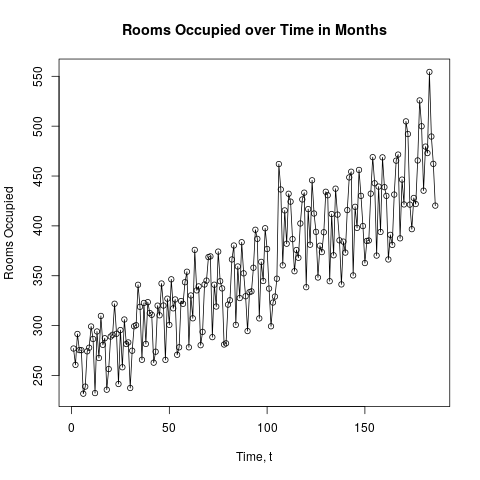
\includegraphics[scale=0.8]{motel.png}
\end{center}
From this plot, we can see that the data does not seem to exhibit constant seasonal variation over time. In the beginning of the time interval, we see that the data seems to be clustered over a range of less than 75 rooms, ranging from just under 300 rooms a night to around 225 rooms a night. At the end of this time interval, we see that the data ranges from around 550 rooms a night to around 425 rooms a night. This is a range of about 125 rooms, which is significantly larger than the other end of the interval. So, we conlcude that a transformation may be the best approach to look at data with a more constant seasonal variation.
\item We now consider the transformation $y^*_t=\ln(y_t)$. After applying this transformation, we look at a plot to see if it has produced a more constant seasonal variation.
\begin{center}
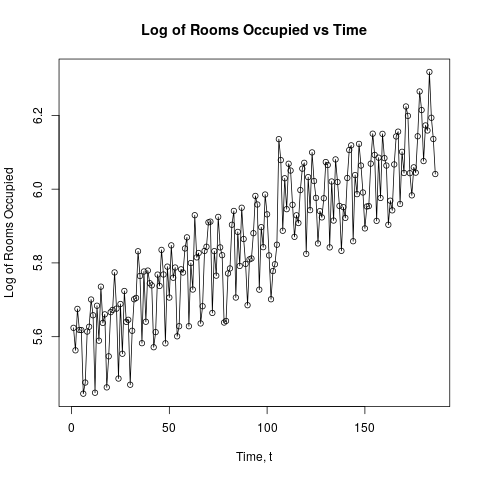
\includegraphics[scale=0.8]{loggedmotel.png}
\end{center}
We see now that the data has a much more constant seasonal variation of about 0.3 at both ends of the time interval. The data has an overall positive linear trend, so we may begin considering a regression model of the data for analysis.
\item We now consider the regression model,
\begin{align*}
y^*_t &= TR_t+SN_t+\varepsilon_t\\
&= \beta_0+\beta_1 t+\beta_2 M_2+\beta_3 M_3+\ldots+\beta_{12} M_{12}+\varepsilon_t
\end{align*}
With $M_i$ being a seasonal dummy variable. Using $R$, we are able to obtain estimates of these $\beta$'s, and the results follow:
\begin{center}
\begin{tabular}{|c|c|}
\hline
$\beta_i$ & Value \\\hline
$\beta_0$ & 5.625 \\
$\beta_1$ & 3.058e-3\\
$\beta_2$ & -8.474e-2\\
$\beta_3$ & 6.629e-02\\
$\beta_4$ & -7.307e-03\\
$\beta_5$ & -5.079e-02\\
$\beta_6$ & -1.945e-01\\
$\beta_7$ & -1.306e-01\\
$\beta_8$ & -7.724e-02\\
$\beta_9$ & -3.248e-02\\
$\beta_{10}$ & 6.767e-02\\
$\beta_{11}$ & 4.062e-02\\
$\beta_{12}$ & -1.730e-01\\\hline
\end{tabular}
\end{center}
As a check of these variables, we test $t=1$ and $t=186$ to see how accurate our model is. For $t=1$, we have,
\[\hat{y}^*_1=5.625+3.058e^-3(1)=5.6281\]
Compared to,
\[y^*_1=5.6240\]
Which is fairly close. We now consider, $t=186$,
\[\hat{y}^*_{186}=5.625+3.058e^-3(186)-1.945e-01=5.9993\]
Compared to,
\[y^*_{186}=6.0410\]
Which, again, is fairly close. So, we see that our model is pretty good.\\
Because we believe that our model is good, we shall now compute a point estimate and interval for July, August, and September of 1995. These values correspond to $t$ values of $187,\ 188,\ 189$ respectively. The predictions follow.
\[\hat{y}^*_{187}=5.625+3.058e^-3(187)-1.306e^-1=6.066414\]
Our interval from R is then,
\[[5.98572,\ 6.14711]\]
These values are in terms of $\ln(y^*)$, so we must in turn undo the log to get the data in useful form. The result is then,
\[\hat{y}_{187}=e^{6.066414}=431.1\]
With a prediction interval of,
\[[e^{5.98572},e^{6.14711}]=[397.7,\ 467.4]\]
Next, we consider August,
\[\hat{y}^*_{188}=5.625+3.058e^-3(188)-7.724e^-2=6.12285\]
With a prediction interval of,
\[[6.042155,\ 6.203546]\]
Undoing the log, we arrive at,
\[\hat{y}_{188}=e^{6.12285}=456.2\]
With interval
\[[420.8,\ 494.5]\]
Finally, we consider September,
\[\hat{y}^*_{189}=5.625+3.058e^-3(189)-3.248e^-2=6.170677\]
With interval,
\[[6.089981,\ 6.251373]\]
Undoing the log, 
\[\hat{y}_{189}=e^{6.170677}=478.5\]
With interval,
\[[441.4,\ 518.7]\]
\item We now compute the first-order autocorrelation of the motel data. Using $R$, and the $acf$ function, we obtain the following plot,
\begin{center}
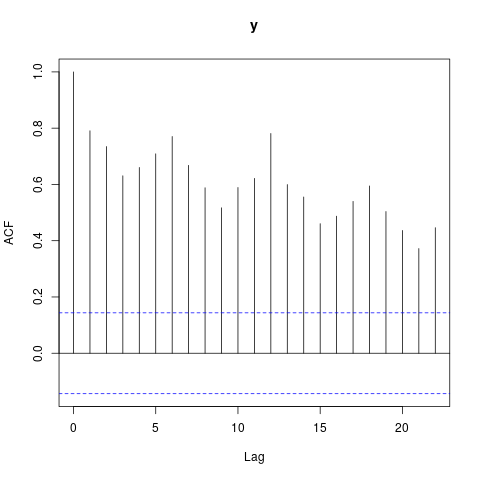
\includegraphics[scale=0.8]{acf.png}
\end{center}
Here, we see that the data looks positively autocorrelated, so we may turn to the computation of the Durbin-Watson test statistic on the simple linear model $y=\beta_0+\beta_1 t$,
\[d=\frac{\sum_{t=2}^n(e_t-e_{t-1})^2}{\sum e_t^2}\]
This value is computed to be,
\[d=1.64255\]
Using $R$. We now perform a Durbin-Watson test to find whether the error term is positively correlated. Usign $R$ again, we compute the $p$-value for this test statistic to be, $p=0.005778$. Thus, we reject the null hypothesis in favor of the alternative, that the true autocorrelation is greater than zero.
\item Now that we have determined that the autocorrelation is greater than zero, we may use ARIMA in $R$ to generate a new model,
\[y^*_t=\beta_0+\beta_1 t+\beta_2 M_2+\beta_3 M_3+\ldots+\beta_{12} M_{12}+\varepsilon_t\]
\[\varepsilon_t=\phi\varepsilon_{t-1}+a_t\]
Using $R$, we estimate the new coefficients to be,
\begin{center}
\begin{tabular}{|c|c|}
\hline
Coefficient & Value \\\hline
$\beta_0$ & 272.2975 \\
$\beta_1$ & 1.0869\\
$\beta_2$ & -29.3315\\
$\beta_3$ & 27.1072\\
$\beta_4$ & -1.0226\\
$\beta_5$ & -18.9682\\
$\beta_6$ & -65.1805\\
$\beta_7$ & -44.3261\\
$\beta_8$ & -29.7758\\
$\beta_9$ & -12.1349\\
$\beta_{10}$ & 26.2514\\
$\beta_{11}$ & 16.2945\\
$\beta_{12}$ & -58.7873\\
$\phi$ & 0.4313\\\hline
\end{tabular}
\end{center}
Now, we may compute our prediction for July of 1995 by computing,
\[\hat{y}_{T+\tau} = b_0+b_1x_{T+\tau,1}+\ldots+b_kx_{T+\tau,k}+\phi e_{T+\tau-1}\]
Here, $\tau=1$ because we have data until June. Thus,
\[e_{T+\tau-1}=e_T=y_T-[b_0+b_1x_{T1}+\ldots]\]
So,
\[e_{186}=y_{186}-\hat{y}_{186}=420.3-412.644=7.6558\]
Our prediction is then,
\[\hat{y}_{187}=b_0+b_1(187)+b_7+\phi*e_{186}=272.2975+1.0869*187-44.3261+7.6558*0.4313=434.528\]
With this point estimate, we may compute the interval,
\[[\hat{y}_{187}\pm z^*s]\]
Here, we may compute that $s=14.04226$, and for a 95\% CI, $z^*=1.96$. Thus, our interval is,
\[[407.005,\ 462.051]\]
\end{enumerate}
\item We now consider the quarterly sales of the board game Oligopoly at a J-Mart variety store. We will use multiplicative decomposition to forcast future quarters sales in Excel. The results of the following calculations are contained in the spreadsheet entitled $problem2$.\\
Before we begin any calculations, we first consider what the data actually looks like,
\begin{center}
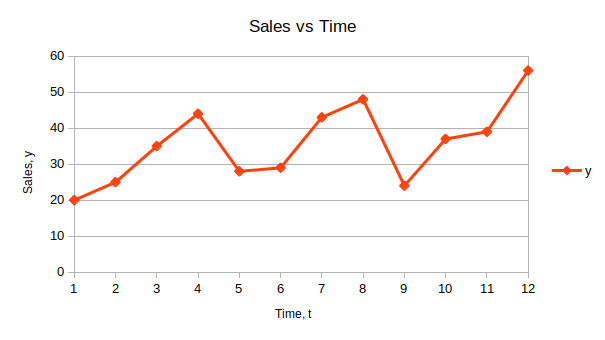
\includegraphics[scale=0.8]{oligopoly.png}
\end{center}
Here, we see that the $y$ data is increasing and periodic, making it a candidiate for decomposition.
\begin{enumerate}
\item First, we compute appropriate four-period moving averages of the data by computing the sum of four consecutive y values and averaging. I.e.
\[M.A._3=\frac{y_1+y_2+y_3+y_4}{4},\ M.A._4=\frac{y_2+y_3+y_4+y_5}{4}\]
And so on. The results of this calculation are contained in Column E of the spreadsheet.
\item We then compute the centered moving averages of the data by averaging consecutive moving averages. I.e.,
\[CMA_3=\frac{MA_3+MA_4}{2},\ CMA_4=\frac{MA_4+MA_5}{2}\]
And so on. The results of this calculation are contained in Column F of the spreadsheet.
\item By construction of our multiplicative model,
\[y_t=TR_t\times SN_t\times CL_t\times IR_t\]
We consider the values of $CMA=TR_t\times CL_t$. Because of this, we may solve for the quantity,
\[SN_t\times IR_t = \frac{y_t}{TR_t\times CL_t}\]
Thus, we may compute our estimations of $sn_t\times ir_t$ by dividing our $y$ data by its corresponding $CMA$ values. This data is contained in Column $G$ of the spreadsheet.
\item We now may compute an average $\bar{sn}_t$ for each quarter by averaging each of the two corresponding data values. We then normalize these values by computing,
\[sn_t=\bar{sn}_t \frac{L}{\sum_t \bar{sn}_t}=\bar{sn}_t \frac{4}{\sum_t \bar{sn}_t}\]
The computations of $\bar{sn}_t$ and the scaling factor are located in the lower regions of Column A of the spreadsheet. The resultant $sn_t$ computations are located in Column H of the spreadsheet.
\item With this seasonal factor computed, we may ``deseasonalize" the data by computing,
\[d_t=\frac{y_t}{sn_t}\]
These computations are contained in Column I of the spreadsheet.
\item We now plot the ``deseasonalized" values over time.
\begin{center}
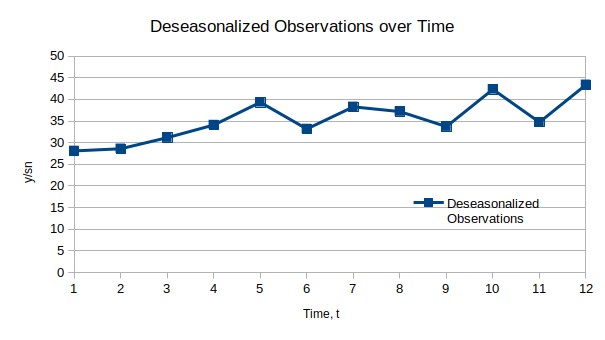
\includegraphics[scale=.8]{deseasonalizedmult.png}
\end{center}
We see that the new deseasonalized data is far more linear than the actual $y$ values from the data set. This trend appears to have positive slope, so we may consider a simple linear model to predict the data with. It is worth noting that there is some variance from true linearity at the end of the time interval, but it does not appear to be too extreme.
\item Assuming linearity from above, we compute the trend,
\[d_t=tr_t=\beta_0+\beta_1 t\]
From the deseasonalized data. Using excel, we compute that the model is,
\[tr_t=28.5593+1.04299t\]
This calculation is in the lower part of column G. Plotting this model over the deseasonalized data,
\begin{center}
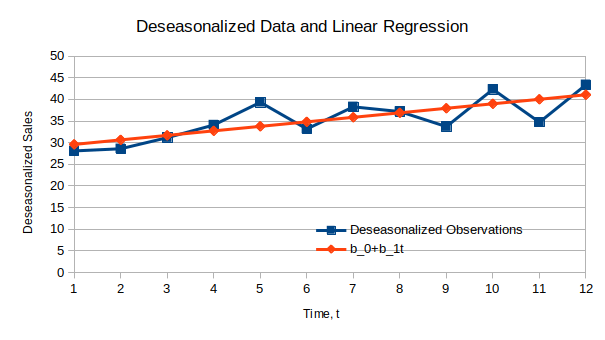
\includegraphics[scale=0.8]{multdeseasonalizedtrend.png}
\end{center}
We see that it fits the deseasonalized data nicely.
\item Finally, we may compute the point forecasts of the sales of Oligopoly in year 4 by copying the appropriate $sn_t$ for each quarter, computing $tr_t$ for each of the quarters, and finally computing our approximation of $\hat{y}_t=tr_t\times sn_t$. These calculations are performed below the columns used above in the spreadsheet, and the results are also highlighted in green.
\begin{center}
\begin{tabular}{|c|c|c|c|}
\hline
Year & Quarter & $t$ & $\hat{y}$ \\\hline
5 & 1 & 13 & 29.985\\
& 2 & 14 & 37.731\\
& 3 & 15 & 49.649\\
& 4 & 16 & 58.402\\\hline
\end{tabular}
\end{center}
\end{enumerate}
\item We now analyze the Oligopoly data using additive decomposition. These results can be found in the spreadsheet $problem3.ods$.
\begin{enumerate}
\item As above, we compute the four period moving averages in Column E.
\item Again, as above, we compute the moving averages in Column F
\item By construction of our additive model,
\[y_t=TR_t+SN_t+CL_t+IR_t\]
We consider the values of $CMA=TR_t+CL_t$. Thus,
\[SN_t+IR_t=y_t-CMA\]
Thus, we may now compute our estimations of $sn_t+ir_t$ by subtracting our $y-CMA$. This computation is performed in Column G of the spreadsheet.
\item In order to compute $sn_t$ for this data, we must first compute the mean, $\bar{sn}_t$ for each of the relevant quarters from the compuation in part (c). First, we compute the means for each quarter in the lower part of Column A. Then, we compute the scaling factor,
\[f=\frac{\sum_t \bar{sn}_t}{L}=\frac{\sum_t \bar{sn}_t}{4}\]
Finally, we may compute,
\[sn_t=\bar{sn}_t-f\]
The results of this scaling are contained in Column H of the spreadsheet.
\item We may now compute the deseasonalized observations for this data by computing,
\[y_t-sn_t=d_t\]
for each of the data points. These results are contained in Column I of the spreadsheet.
\item We now look at the deseasonalized data in plot form,
\begin{center}
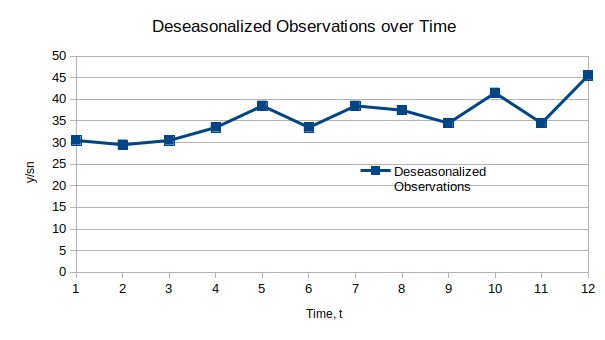
\includegraphics[scale=0.8]{adddeseasonal.png}
\end{center}
We see from this plot that the deseasonalized data exhibits a positive linear trend as before, with a similar divergence at the end of the time interval to the multiplicative decomposition.
\item Assuming linearity from before, we now compute the model,
\[d_t=tr_t=\beta_0+\beta_1t\]
Using Excel, we compute the model to be,
\[tr_t=28.98485+1.02797t\]
Plotting this regression model over the deseasonalized data, we see that it is indeed a good fit.
\begin{center}
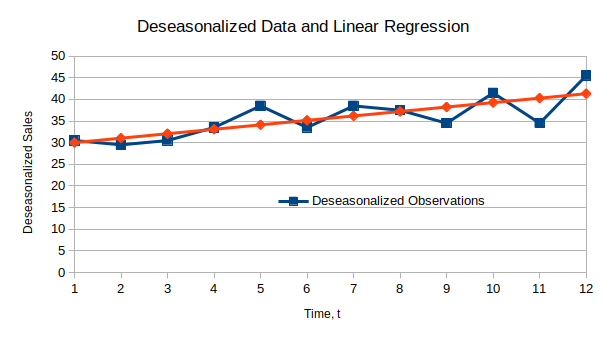
\includegraphics[scale=0.8]{addregression.png}
\end{center}
\item Finally, we may compute the point forecasts of the sales of Oligopoly in year 4 by copying the appropriate $sn_t$ for each quarter, computing $tr_t$ for each of the quarters, and finally computing our approximation of $\hat{y}_t=tr_t + sn_t$. These calculations are performed below the columns used above in the spreadsheet, and the results are also highlighted in green.
\begin{center}
\begin{tabular}{|c|c|c|c|}
\hline
Year & Quarter & $t$ & $\hat{y}$ \\\hline
5 & 1 & 13 & 31.8485\\
& 2 & 14 & 38.8765\\
& 3 & 15 & 48.9044\\
& 4 & 16 & 55.9324\\\hline
\end{tabular}
\end{center}
\item We now compare the two models to decide which fits the data better. First, let us consider the over lay of our computed $\hat{y}$ values versus the true $y$ values from the data for each model.
\begin{center}
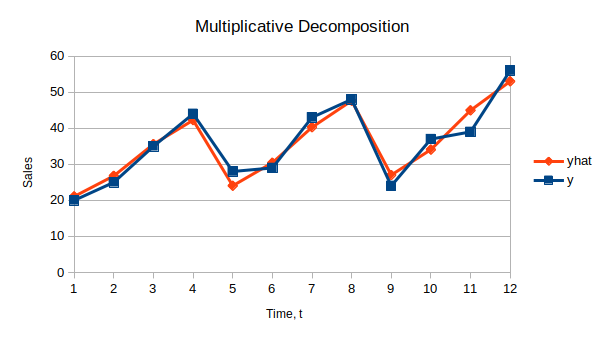
\includegraphics[scale=0.8]{multyhat.png}
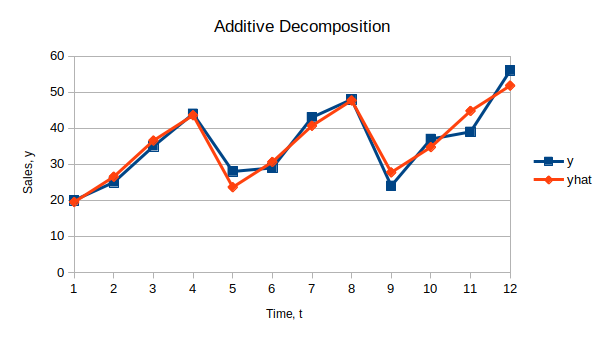
\includegraphics[scale=0.8]{addhat.png}
\end{center}
Simply looking at these two plots, it is not readily apparent which is better. They are clearly almost identical to the true values of $y$, which is a good thing. We now consider,
\begin{center}
\begin{tabular}{|c|c|}
\hline
Decomposition & SSE\\\hline
Multiplicative & 95.090\\
Additive & 102.555\\\hline
\end{tabular}
\end{center}
So, again, we see that the models are nearly identical, with the Multiplicative decomposition narrowly beating out the additive for accuracy over the experimental region. Finally, we return to our original plot of the data,
\begin{center}
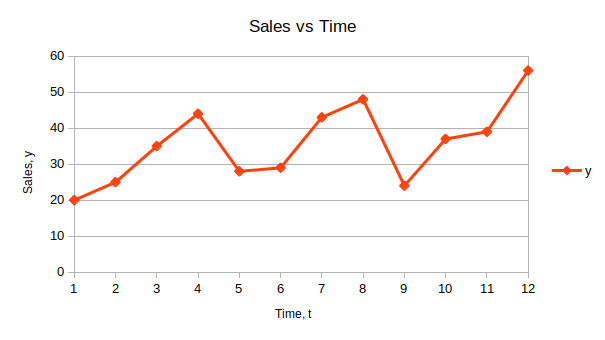
\includegraphics[scale=0.8]{oligopoly.png}
\end{center}
We know that time series with constant seasonal variation are better suited for additive decomposition, while those with changing seasonal variation are better suited for multiplicative decomposition. Looking at the data, we see that the seasonal variation seems to be vaguely increasing, but there are only a few data points for each season, which makes the analysis challenging. In the end, we conclude that the multiplicative model is better, but the additive model is still fairly good given the data available to us.
\end{enumerate}
\item We shall now analyze the quarterly sales of the Tiger Sports Drink over the last eight years.
\begin{enumerate}
\item First, we plot the time series data.
\begin{center}
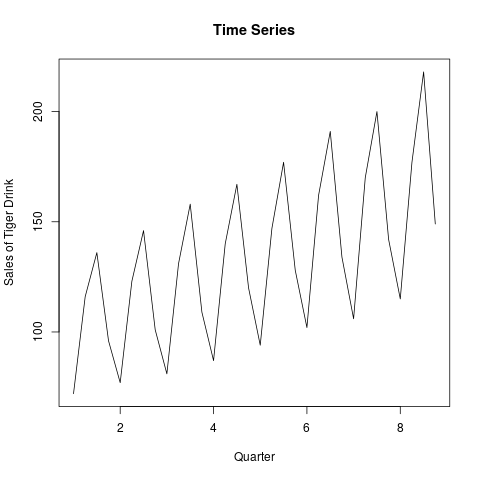
\includegraphics[scale=0.8]{tigersales.png}
\end{center}
Looking at this plot, we clearly see that the seasonal pattern is increasing as time increases.  So, we shall employ a multiplicative Holt-Winters model to forecast the sales. Using the parameters, $\alpha=0.2,\ \beta=0.1,\ \gamma=0.1$, $R$ computes the initial states to be,
\begin{center}
\begin{tabular}{|c|c|}
\hline
Parameter & Value\\\hline
$l_0$ & 100.301\\
$b_0$ & 1.4349\\
$sn_{-3}$ & 0.8967\\
$sn_{-2}$ & 1.2982\\
$sn_{-1}$ & 1.1016\\
$sn_0$ & 0.7035\\\hline
\end{tabular}
\end{center}
This model also has $MSE=129.9333$.
\item We now use $R$ to optimize the values of $\alpha,\ \beta,\ \gamma$. The resultant parameters are,
\[\alpha=0.2046\]
\[\beta=0.0316\]
\[\gamma=0.0001\]
This model has a $MSE=105.7211$. With this model generated, we may compute a point forecast and interval for the first quarter of year 9. The result is, 
\[\hat{y}_{q1}=119.5340\]
\[PI=[115.9068,\ 123.1611]\]
\item We shall now take the log of the data, and perform the same analysis as before.
\begin{enumerate}
\item Using the parameters, $\alpha=0.2,\ \beta=0.1,\ \gamma=0.1$, $R$ computes the initial states to be,
\begin{center}
\begin{tabular}{|c|c|}
\hline
Parameter & Value\\\hline
$l_0$ & 4.5893\\
$b_0$ & 0.0143\\
$sn_{-3}$ & 0.0838\\
$sn_{-2}$ & 0.285\\
$sn_{-1}$ & 0.1244\\
$sn_0$ & -0.3255\\\hline
\end{tabular}
\end{center}
This model has, $MSE=0.0060$.
\item Now, we will let $R$ optimize the parameters, which results in,
 \[\alpha=0.1721\]
\[\beta=0.0001\]
\[\gamma=0.0001\]
This model has $MSE=0.00496$.
With this model, we may predict the first quarter of year 9. We compute,
\[\hat{y}_{q1}=4.796579\Rightarrow \hat{y}=e^{4.796579}=121.095\]
\[PI=[4.768407,\ 4.824752]\Rightarrow PI=[e^{4.768407},\ e^{4.824752}]=[117.732,\ 124.556]\]
\end{enumerate}
\item Comparing these two models, we may conclude that the Additive model does a better job. Not only does it have the smallest MSE values, it also produces the tighter of the two prediction intervals, implying that it is slightly more accurate.
\end{enumerate}
\item We now look at the house sales data for one family houses. Computing a simple linear regression on the first 12 months of the data set, and then using smoothing parameters $\alpha=0.2$ and $\beta=0.1$, we run Holt's trend corrected smoothing. With this model we obtain the following values,
\begin{align*}
SSE &= 8005.074 \\
MSE &= 74.12106\\
s &= 8.6902\\
MAD &= 6.93675\\
MAPE &= 13.6724\\
\end{align*}
\item Allowing a solver to optimize the values of $\alpha,\ \beta$, we arrive at the values of,
\[\alpha=1\]
\[\beta=.02407\]
Which result in a value of $SSE=4392.6834$
\item Using the computed coefficients of $l_{108}$ and $b_{108}$, we compute the point forecasts,
\begin{align*}
y_{109} &= l_{108}+b_{108}\\
&=41.5573\\
y_{110} &= l_{108}+2b_{108}\\
&=41.1146
\end{align*}
The intervals for these predictions are,
\[[y_{109}\pm z^*s]=[28.9399,\ 54.1746]\]
\[[y_{110}\pm z^*s\sqrt{1+\alpha^2(1+\beta)^2}]=[23.0549,\ 59.1742]\]
\end{enumerate}
\end{document}
